\documentclass{article}
\usepackage[letterpaper, top=0.15in, left=0.5in, right=0.5in, bottom=1in]{geometry}
\usepackage{amsmath, amssymb}
\usepackage{tcolorbox}
\usepackage[dvipsnames]{xcolor}
\usepackage{ifthen}
\tcbuselibrary{listings,breakable}
\usepackage{float} % Allows precise placement of floating objects
\usepackage{tikz} % Core TikZ package
\usepackage{pgfplots} % For statistical plots
\pgfplotsset{compat=1.18} % Ensure compatibility

\usetikzlibrary{positioning, shapes, calc, backgrounds, decorations.pathreplacing, arrows.meta, plotmarks}

\usepackage{comment}
\setlength{\parindent}{0pt} % remove indentation in the whole document

% Define a new command for a centered floating blank text box
\newcommand{\blankbox}[2][3cm]{%
    \vspace{-0.5em}
    \begin{figure}[H]
        \makebox[\linewidth]{% Ensures the box extends to full line width
            \begin{tcolorbox}[
                colback=white, 
                colframe=black, 
                width=#2, % Adjusting for A4 paper margins
                height=#1,
                boxrule=0.2mm
            ]
            \end{tcolorbox}
        }
    \end{figure}
    \vspace{-1em}
}
% Define a new boolean for showing or hiding answers
\newboolean{showanswers}
\setboolean{showanswers}{false}  % Set to true to show answers, false to hide answers

% Define the command to conditionally display answers
\newcommand{\answer}[1]{
    \ifthenelse{\boolean{showanswers}}{
        \begingroup
        \color{MidnightBlue}
        \begin{tcolorbox}[colback=white, colframe=MidnightBlue, title=Solution, fonttitle=\bfseries, breakable, fontupper=\color{MidnightBlue}]
        #1
        \end{tcolorbox}
        \endgroup
    }{}
}

\title{Midterm Practice Problem Set - POL201.01}
\author{Version 2 - 03/10/2025}
\date{}

\begin{document}

\maketitle

\textbf{DISCLAIMER}: This practice problem set serves as a representative sample of the types of questions that will appear on the actual exam. However, since the midterm is limited to approximately 90 minutes, it will be significantly shorter than this practice version. The goal of this practice problem set is to give you ample opportunity to reinforce your understanding and refine your problem-solving skills.

\textbf{NOTE}: I will post the solutions to the problem set questions Monday 03/10 (pm). So, it is strongly recommended that you start working on the questions well before the solutions are posted. Also, just reading through the solutions without trying to attempt the problems first is a poor studying strategy. Always try to solve the problems first, then use the solutions to check your work.

\section*{Section 1: Introduction to Data}

\noindent\textbf{Instructions:}  
For each statement below, circle \texttt{True} or \texttt{False}, then provide a brief justification explaining your answer.

\vspace{0.5cm}

\noindent \textbf{Study Context:}  
A team of researchers surveyed a sample of farmers across various regions to understand their financial habits, experiences with government loans for implementing green economy technologies, and attitudes toward sustainable agricultural practices. The researchers did not assign any treatments or intervene in any way; they simply collected self-reported data from participants over a single time period.

\vspace{0.5cm}
\noindent Consider the first few rows of the collected sample dataset:

\begin{center}
\small
\begin{tabular}{c|c|c|c|c|c|c}
\textbf{Business ID} & \textbf{Owner Age} & \textbf{Revenue} & \textbf{Loan Approved} & \textbf{Years in Business} & \textbf{Region} & \textbf{Business Type}\\
\hline
1 & 52 & 180000 & Yes & 12 & West & Retail\\
2 & 37 & 95000 & No & 5 & East & Service\\
3 & 45 & 200000 & Yes & 15 & South & Manufacturing\\
4 & 40 & 120000 & No & 8 & South & Retail\\
5 & 50 & 170000 & Yes & 10 & West & Technology\\
\vdots & \vdots & \vdots & \vdots & \vdots & \vdots & \vdots
\end{tabular}
\normalsize
\end{center}

\begin{enumerate}

\item \textbf{Statement A:} Owner Age is a continuous numerical variable, while Business Type is an ordinal categorical variable.

    \noindent
    \texttt{True} \quad \texttt{False}

    \blankbox[4cm]{1.1\textwidth} % A box with 4cm height and full text width
    \answer{
    \textbf{False.} Owner Age is indeed a continuous numerical variable because it can take any value within a range. However, Business Type is a \textbf{nominal} categorical variable because it consists of distinct categories (Retail, Service, Manufacturing, etc.) without a meaningful order.
    }

\item \textbf{Statement B:} The dataset above represents an \textit{experimental} study capable of establishing causation.

    \noindent
    \texttt{True} \quad \texttt{False}
    
    \blankbox[4cm]{1.1\textwidth} % A box with 4cm height and full text width
    \answer{
    \textbf{False.} This is an observational study, as the researchers simply collected self-reported data without assigning businesses to treatment or control groups. \textbf{No random assignment} means causation cannot be established—only associations can be identified.
    }

\item \textbf{Statement C:} Assume each member of the population had the same probability of being selected in the sample data. \emph{Therefore}, the results from this sample can be generalized to the larger population of small business owners.

    \noindent
    \texttt{True} \quad \texttt{False}
    
    \blankbox[4cm]{1.1\textwidth} % A box with 4cm height and full text width
    \answer{
    \textbf{True.} This matches the definition of \textbf{simple random sampling}, where every member of the population has an equal chance of being selected. When a sample is truly random, it is \textbf{representative} of the population, allowing for valid generalizations. 
    }


\item \textbf{Statement D:} If Loan Approval and Years in Business are strongly associated in the dataset, that guarantees that having more years in business causes higher loan approval rates.

    \noindent
    \texttt{True} \quad \texttt{False}
    
    \blankbox[4cm]{1.1\textwidth} % A box with 4cm height and full text width
    \answer{
    \textbf{False.} A strong association between \textbf{Loan Approval} and \textbf{Years in Business} does not imply causation. The relationship might be influenced by \textbf{confounding variables} such as \textbf{credit score, business revenue, or industry trends}. Correlation does not equal causation.
    }

\item \textbf{Statement E:} Suppose that researchers collected this data only using online surveys sent to businesses that had previously interacted with financial institutions. If the sampling was random within this group, there is no chance of sampling bias.

    \noindent
    \texttt{True} \quad \texttt{False}
    
    \blankbox[4cm]{1.1\textwidth} % A box with 4cm height and full text width
    \answer{
    \textbf{False.} Even though selection within the sample was random, \textbf{sampling bias} can still exist because the overall \textbf{sampling procedure is biased} since inception—only businesses with previous financial institution interactions were included. Businesses that rely on alternative funding or are new might be underrepresented, leading to \textbf{statistical bias} (specifically, \emph{coverage bias}).
    }

\end{enumerate}

%%%%%%%%%%%%%%%%%%%%%%%%%%%%%%%%%%%%%%%%%%%%%%%%%%%%%%%%%%%%%%%%%%%%%%%%%%%%%%%%%%%%
\newpage

\section*{Section 2: Describing and Summarizing Data}

\noindent
In political science, analyzing the frequency of discussions about political events can provide insights into civic engagement and public opinion dynamics. Below is a dataset representing the number of times a random sample of 18 high school students engaged in political discussions with friends over the past month.
\[
\{\,1,1,1,1,1,\;\,2,2,2,2,\;\,3,3,3,\;\,4,4,\;\,5,\;\,6,6,\;\,7\}.
\]
\noindent
For this dataset, the following aggregates or summaries are provided:
\[
\sum x_i = 54, \quad \sum (x_i - \bar{x})^2 = 64, \quad n = 18
\]

\begin{comment}
{
    "sum_x": ,
    "sum_x_squared": 226,
    "sum_x_minus_mean_squared": 64.0,
    "n": 18,
    "Q1": 1,
    "Q2": 2.5,
    "Q3": 4
}

\end{comment}


\begin{figure}[H]
\begin{center}
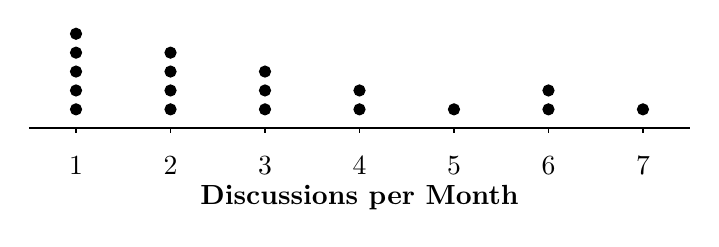
\begin{tikzpicture}[x=1.2cm, y=1.2cm]

    % Draw horizontal axis from 0.5 to 7.5
    \draw[thick] (0.5,0) -- (7.5,0);

    % Tick marks and x-axis labels
    \foreach \x in {1,2,3,4,5,6,7} {
        \draw (\x, 0) -- (\x, -0.05);    % tick mark
        \node[below] at (\x, -0.2) {\x}; % x-axis label
    }
    \node[below] at (4, -0.5) {\textbf{Discussions per Month}};

    %-------------------------------
    % Plot the 20 data points
    % (Manual stacking for each repeated value)
    %-------------------------------

    % 1's (5 occurrences)
    \draw[fill] (1, 0.2) circle (2pt);
    \draw[fill] (1, 0.4) circle (2pt);
    \draw[fill] (1, 0.6) circle (2pt);
    \draw[fill] (1, 0.8) circle (2pt);
    \draw[fill] (1, 1.0) circle (2pt);

    % 2's (4 occurrences)
    \draw[fill] (2, 0.2) circle (2pt);
    \draw[fill] (2, 0.4) circle (2pt);
    \draw[fill] (2, 0.6) circle (2pt);
    \draw[fill] (2, 0.8) circle (2pt);

    % 3's (3 occurrences)
    \draw[fill] (3, 0.2) circle (2pt);
    \draw[fill] (3, 0.4) circle (2pt);
    \draw[fill] (3, 0.6) circle (2pt);

    % 4's (2 occurrences)
    \draw[fill] (4, 0.2) circle (2pt);
    \draw[fill] (4, 0.4) circle (2pt);

    % 5's (1 occurrences)
    \draw[fill] (5, 0.2) circle (2pt);

    % 6's (2 occurrences)
    \draw[fill] (6, 0.2) circle (2pt);
    \draw[fill] (6, 0.4) circle (2pt);

    % 7's (1 occurrences)
    \draw[fill] (7, 0.2) circle (2pt);
\end{tikzpicture}
\caption{Dot Plot of Students' Discussions per Month ($X$)}
\end{center}
\end{figure}

\vspace{-3em}
\subsection*{Questions}
Thoroughly justify all your answers. 

\begin{enumerate}
    \item \textbf{Measures of Central Tendency:}  
    \begin{enumerate}
      \item[(a)] Calculate the \emph{mean} number of political discussions per student.  
      \item[(b)] Find the \emph{median} number of discussions.  
      \item[(c)] Identify the \emph{mode}.  
      \item[(d)] Compare and interpret these measures and comment on any qualitative differences you observe.
    \end{enumerate}
    \blankbox[8cm]{1.1\textwidth} % A box with 4cm height and full text width
    \answer{ } % ANSWER GOES HERE

\newpage %%%%%%%%%%%%%%%%%%%%%%%%%%%%%%%%%%%%%%%%%%%%%%%%%%%%%%%%
    \item \textbf{Measures of Spread:}  
    \begin{enumerate}
      \item[(a)] Compute the \emph{range} of the data.  
      \item[(b)] Determine the \emph{interquartile range} (IQR).  
      \item[(c)] Calculate the sample \emph{standard deviation}.
      \item[(d)] Compare and interpret these measures and comment on any qualitative differences you observe.
    \end{enumerate}
    \blankbox[8cm]{1.1\textwidth} % A box with 4cm height and full text width
    \answer{ } % ANSWER GOES HERE
    
    \item \textbf{Skewness and Outliers:}  
    \begin{enumerate}
      \item[(a)] What can you infer about the skewness of the data by comparing the mean and median? Is your answer consistent with a visual inspection of the shape of the distribution?
      \item[(b)] Are there any data points you might consider as outliers in this set? Justify your answer using the $\pm1.5\cdot IQR$ rule of thumb to classify outliers.
    \end{enumerate}
    \blankbox[5cm]{1.1\textwidth} % A box with 4cm height and full text width
    \answer{ } % ANSWER GOES HERE

    \item \textbf{Impact of New Data:}  
    Suppose a new student joins the class, reporting 15 political discussions per month. 
    \begin{enumerate}
      \item[(a)] Predict qualitatively how adding this data point would affect the \emph{mean} and \emph{median}.  
      \item[(b)] Between the mean and the median, which measure of central tendency is more robust when a new extreme value is added? Explain why.
    \end{enumerate}
    \blankbox[5cm]{1.1\textwidth} % A box with 4cm height and full text width
    \answer{ } % ANSWER GOES HERE
    
\end{enumerate}

%%%%%%%%%%%%%%%%%%%%%%%%%%%%%%%%%%%%%%%%%%%%%%%%%%%%%%%%%%%%%%%%%%%%%%%%%%%%%%%%%%%%
\newpage

\section*{Section 3: Probability Rules}

\noindent\textbf{Instructions:}  
For each of the following problems, write down the correct probability rule you applied and show your calculations.

\begin{enumerate}

    \item \textbf{Question A:}  
    A political survey finds that 40\% of voters support Candidate A, 35\% support Candidate B, and 25\% are undecided. If one voter is selected at random, what is the probability that they support either Candidate A or Candidate B?
    
    \blankbox[4cm]{1.1\textwidth}  
    \answer{
    Using the \textbf{addition rule for mutually exclusive events}:  
    \[
    P(A \text{ or } B) = P(A) + P(B) = 0.40 + 0.35 = 0.75
    \]  
    The probability that a randomly selected voter supports either Candidate A or Candidate B is \textbf{0.75}.
    }

    \item \textbf{Question B:}  
    A school district surveyed 2,000 randomly selected students from two high schools: 1,200 from School A and 800 from School B. Of these, 500 students from School A and 400 students from School B participated in at least one extracurricular activity.\\ Is the following statement \texttt{True} or \texttt{False} (justify)? ``\emph{A randomly selected student from School A is more likely to participate in at least one extracurricular activity than a randomly selected student from School B.}"

    \blankbox[4cm]{1.1\textwidth}  
    \answer{
    }

    \item \textbf{Question C:}  
    A university study finds that 20\% of students do not own a laptop, and among all students. Additionally, the study finds that 48\% own both a laptop and a tablet. If a student is randomly selected and found to own a laptop, what is the probability that they also own a tablet?
    
    \blankbox[4cm]{1.1\textwidth}  
    \answer{
    Using the \textbf{conditional probability formula}:  
    \[
    P(\text{Tablet} | \text{Laptop}) = \frac{P(\text{Tablet and Laptop})}{P(\text{Laptop})}
    \]  
    Given \( P(\text{Tablet and Laptop}) = 0.48 \) and \( P(\text{Laptop}) = 0.80 \),  
    \[
    P(\text{Tablet} | \text{Laptop}) = \frac{0.48}{0.80} = 0.60
    \]  
    The probability that a student owns a tablet given that they own a laptop is \textbf{0.60}.
    }
    \item \textbf{Question D:}  
    Suppose the probability that a randomly selected registered voter will turn out to vote in an election is 0.65. If two registered voters are randomly selected, what is the probability that both of them will vote?
    
    \blankbox[4cm]{1.1\textwidth}  
    \answer{
    Since voting behavior of one voter is assumed to be \textbf{independent} of the other, we use the \textbf{multiplication rule for independent events}:  
    \[
    P(A \text{ and } B) = P(A) \times P(B) = 0.65 \times 0.65 = 0.4225
    \]  
    The probability that both voters will turn out to vote is \textbf{0.4225}.
    }

    \item \textbf{Question E:}  
    A research study finds that 50\% of students take a statistics course, 40\% take a political science course, and 20\% take both. What is the probability that a randomly selected student takes either a statistics or a political science course?
    
    \blankbox[4cm]{1.1\textwidth}  
    \answer{
    Using the \textbf{general addition rule}:  
    \[
    P(A \text{ or } B) = P(A) + P(B) - P(A \text{ and } B)
    \]  
    \[
    P(\text{Statistics or Political Science}) = 0.50 + 0.40 - 0.20 = 0.70
    \]  
    The probability that a student takes either a statistics or political science course is \textbf{0.70}.
    }

    \item \textbf{Question F:}  
    A survey shows that 30\% of people get their news from social media, 50\% from television, and 20\% from newspapers. The probability of misinformation being shared is 0.25 for social media, 0.10 for television, and 0.05 for newspapers. What is the overall probability that a randomly chosen person encounters misinformation?
    
    \blankbox[4cm]{1.1\textwidth}  
    \answer{
    Using the \textbf{law of total probability}:  
    \[
    P(\text{Misinformation}) = P(M | SM)P(SM) + P(M | TV)P(TV) + P(M | NP)P(NP)
    \]  
    \[
    = (0.25 \times 0.30) + (0.10 \times 0.50) + (0.05 \times 0.20)
    \]  
    \[
    = 0.075 + 0.05 + 0.01 = 0.135
    \]  
    The probability that a randomly chosen person encounters misinformation is \textbf{0.135}.
    }

    \item \textbf{Question G:}  
    An AI tool is designed to detect misinformation in online articles. It analyzes an article and predicts whether it contains false information. The tool has the following performance characteristics:
    \begin{itemize}
        \item If an article truly contains misinformation, the AI correctly flags it 95\% of the time (true positive rate).
        \item If an article is actually truthful, the AI incorrectly flags it as misinformation 15\% of the time (false positive rate).
        \item Before analyzing an article, the estimated probability that any randomly selected article contains misinformation is 0.2 (the prior probability).
    \end{itemize}
    If the AI flags an article as misinformation, what is the probability that the article is actually false?
    
    \blankbox[4cm]{1.1\textwidth}  
        \answer{
        By Bayes' Theorem:
        \[
        P(M | F) = \frac{P(F | M) P(M)}{P(F)}
        \]
        where:
        \[
        P(F) = P(F | M) P(M) + P(F | \neg M) P(\neg M)
        \]
        
        \[
        = (0.95 \times 0.2) + (0.15 \times 0.8) = 0.19 + 0.12 = 0.31
        \]
        
        Thus:
        \[
        P(M | F) = \frac{0.19}{0.31} \approx 0.613
        \]
        
        Final answer: **61.3\%**.
        }
        
        
    \item \textbf{Question H:}  
    A political survey finds that 24\% of voters support Candidate X, 15\% support Candidate Y, and 61\% are undecided. If one voter is selected at random, and given this voter is not undecided, what is the probability that they prefer Candidate X?
    
    \blankbox[4cm]{1.1\textwidth}  
    \answer{
    Using the \textbf{addition rule for mutually exclusive events}, we first determine the probability of a voter supporting either Candidate X or Candidate Y:
    
    \[
    P(X \text{ or } Y) = P(X) + P(Y) = 0.24 + 0.15 = 0.39
    \]
    
    Next, applying the \textbf{conditional probability formula}:
    
    \[
    P(X | \text{Not Undecided}) = \frac{P(X)}{P(X \text{ or } Y)}
    \]
    
    \[
    = \frac{0.24}{0.39} \approx 0.615
    \]
    
    Thus, the probability that a voter prefers Candidate X given that they are not undecided is \textbf{61.5\%}.
    }
    

\end{enumerate}

%%%%%%%%%%%%%%%%%%%%%%%%%%%%%%%%%%%%%%%%%%%%%%%%%%%%%%%%%%%%%%%%%%%%%%%%%%%%%%%%%%%%
%%%%%%%%%%%%%%%%%%%%%%%%%%%%%%%%%%%%%%%%%%%%%%%%%%%%%%%%%%%%%%%%%%%%%%%%%%%%%%%%%%%%
\newpage
\section*{Section 4: Probability - Vote Miscounting Puzzle}

\noindent\textbf{Instructions:}  
For each of the following problems, write down the correct probability rule you applied and show your calculations. \underline{Note}: Do questions (a) and (b). The rest are given as a challenge. 

\begin{enumerate}
    \item \textbf{Question: Probability Puzzle on Vote Miscounting}

    In an election, Candidate \( A \) receives 55\% of the votes (i.e., $P(A)=0.55$), and Candidate \( B \) receives 45\% of the votes (i.e., $P(B)=0.45$). However, due to potential miscounting ($M$), each vote has a 10\% probability of being counted incorrectly. This means:
    \begin{itemize}
        \item A vote for \( A \) has a 10\% probability of being miscounted as a vote for \( B \) (i.e., \( P(M | A) = 0.10 \)), and a 90\% probability of being counted correctly (i.e., \( P(M^c | A) = 0.90 \)).
        \item A vote for \( B \) has a 10\% probability of being miscounted as a vote for \( A \) (i.e., \( P(M | B) = 0.10 \)), and a 90\% probability of being counted correctly (i.e., \( P(M^c | B) = 0.90 \)).
    \end{itemize}

    Using the appropriate probability rules, answer the following:

    \begin{enumerate}
        \item[(a)] What is the probability that a randomly selected vote is counted correctly?  
        \textit{Tip: Use the law of total probability.}
        \blankbox[5cm]{1.1\textwidth}

        \item[(b)] What is the probability that a randomly selected vote is miscounted?  
        \textit{Tip: Use the complement rule.}
        \blankbox[5cm]{1.1\textwidth}

        \item[(c)] (\textbf{Challenge Question}) What is the probability that a randomly selected vote was truly cast for Candidate \( A \) before miscounting, denoted \( P(A^*) \)?  
        \textit{Tip: Compute \( P(A^*) \) by considering both correctly counted votes for \( A \) and votes miscounted from \( B \) to \( A \). Use the following version of the law of total probability:}
        \begin{align*}
         P(A^*) &= P(\text{Correctly Counted for A}) + P(\text{Miscounted for B})   \\ 
             & = P(M^c \cap A) + P(M \cap B) = P(M^c | A) P(A) + P(M | B) P(B).
        \end{align*} \vspace{-2em}
        \blankbox[5cm]{1.1\textwidth}

        \item[(d)] (\textbf{Challenge Question}) What is the probability that a randomly selected vote was truly cast for Candidate \( B \) before miscounting, denoted \( P(B^*)  \)?  
        \textit{Tip: Compute \( P(B^*) \) by considering both correctly counted votes for \( B \) and votes miscounted from \( A \) to \( B \). Use the following version of the law of total probability:}
        \begin{align*}
         P(B^*) &= P(\text{Correctly Counted for B}) + P(\text{Miscounted for A})   \\ 
             &= P(M^c \cap B) + P(M \cap A) = P(M^c | B) P(B) + P(M | A) P(A).
        \end{align*} \vspace{-2em}
        \blankbox[5cm]{1.1\textwidth}

        \item[(e)] (\textbf{Challenge Question}) Given your calculations of \( P(A^*) \) and \( P(B^*) \), does vote miscounting change the expected winner of the election?  
        \textit{Tip: Compare \( P(A^*) \) and \( P(B^*) \) to determine if the winner remains the same.}
        \blankbox[5cm]{1.1\textwidth}

        \item[(f)] (\textbf{Challenge Question}) Suppose instead that the probability of miscounting is some unknown value \( \theta \), where \( P(M | A) = P(M | B) = \theta \).  
        What is the largest value of \( \theta \) for which Candidate \( A \) remains the expected winner?  
        \textit{Hint:}
        \begin{enumerate}
            \item[(i)] Express \( P(A^*) \) and \( P(B^*) \) in terms of \( \theta \).
            \item[(ii)] Solve for \( \theta \) when \( P(A^*) = P(B^*) \).
            \item[(iii)] Interpret the result: What does this tell you about the sensitivity of the election outcome to miscounting?
        \end{enumerate}
        \blankbox[5cm]{1.1\textwidth}

    \end{enumerate}

    \answer{
    \begin{align*}
    P(M^c) &= P(M^c | A) P(A) + P(M^c | B) P(B) \\
    &= (0.90 \times 0.55) + (0.90 \times 0.45) \\
    &= 0.495 + 0.405 \\
    &= 0.90.
    \end{align*}

    \begin{align*}
    P(M) &= 1 - P(M^c) \\
    &= 1 - 0.90 \\
    &= 0.10.
    \end{align*}

    \begin{align*}
    P(A^*) &= P(M^c | A) P(A) + P(M | B) P(B) \\
    &= (0.90 \times 0.55) + (0.10 \times 0.45) \\
    &= 0.495 + 0.045 \\
    &= 0.54.
    \end{align*}

    \begin{align*}
    P(B^*) &= P(M^c | B) P(B) + P(M | A) P(A) \\
    &= (0.90 \times 0.45) + (0.10 \times 0.55) \\
    &= 0.405 + 0.055 \\
    &= 0.46.
    \end{align*}

    \begin{align*}
    A^* &= 0.54, \quad B^* = 0.46.
    \end{align*}

    Since \( A^* > B^* \), \textbf{Candidate \( A \) still wins}. The key takeaway is that as long as Candidate \( A \)'s original lead is \textbf{greater than the probability of miscounting}, the final result remains unchanged.
    }
\end{enumerate}

%%%%%%%%%%%%%%%%%%%%%%%%%%%%%%%%%%%%%%%%%%%%%%%%%%%%%%%%%%%%%%%%%%%%%%%%%%%%%%%%%%%%
%%%%%%%%%%%%%%%%%%%%%%%%%%%%%%%%%%%%%%%%%%%%%%%%%%%%%%%%%%%%%%%%%%%%%%%%%%%%%%%%%%%%

\newpage
\section*{Section 5: Linear Combination of Random Variables}

\noindent\textbf{Instructions:}  
For each of the following problems, apply the appropriate statistical concepts related to linear transformations of random variables, expectations, variances, and probability distributions. Clearly show all steps in your calculations.

\begin{enumerate}
    \item \textbf{Question: Sales Commissions and Expected Earnings}

    Alex works as a salesperson for two different companies:
    \begin{itemize}
        \item \textbf{Job A:} Sales revenue in a given week is represented by the discrete random variable \( X \), with expectation \( E[X] = 5000 \) and variance \( V(X) = 1,000,000 \).
        \item \textbf{Job B:} Sales revenue in a given week is represented by the discrete random variable \( Y \), with expectation \( E[Y] = 3000 \) and variance \( V(Y) = 400,000 \).
        \item Alex receives a \textbf{commission} of \textbf{5\%} on sales from \textbf{Job A} and \textbf{10\%} on sales from \textbf{Job B}.
    \end{itemize}

    Alex’s total commission earnings are given by:

    \[
    Z = 0.05X + 0.10Y
    \]

    Answer the following:

    \begin{enumerate}
        \item[(a)] Compute the \textbf{expected total commission earnings} \( E[Z] \).
        \blankbox[5cm]{1.1\textwidth}

        \item[(b)] Compute the \textbf{variance of total commission earnings} \( V(Z) \), assuming that \( X \) and \( Y \) are independent.
        \blankbox[5cm]{1.1\textwidth}

        \item[(c)] Compute the \textbf{standard deviation of \( Z \)}, denoted \( \sigma_Z \).
        \blankbox[5cm]{1.1\textwidth}

        \item[(d)] \textbf{In terms of standard deviation units, how far is \( Z = 630.62 \) from the mean?}
        \begin{itemize}
            \item \emph{Hint: Compute the \textbf{Z-score}:}
            \[
            Z_{\text{score}}(630.62) = \frac{630.62 - E[Z]}{\sigma_Z}
            \]
        \end{itemize}
        \blankbox[5cm]{1.1\textwidth}

        \item[(e)] \textbf{Now assume \( Z_{\text{score}} \) follows a standard normal distribution. Compute the probability that Alex earns more than \$630.62 in commissions, i.e., find \( P(Z_{\text{score}} > Z_{\text{score}}(630.62)) \).}  
        \begin{itemize}
            \item \emph{Hint: Use the \textbf{standard normal CDF table} below to find the cumulative probability \( P(Z_{\text{score}} \leq Z_{\text{score}}(630.62)) \).}
        \begin{center}
        \begin{tabular}{c|c c c c c c c}
        \( Z_{\text{score}} \)  & -3  & -2  & -1  &  0  &  1  &  2  &  3  \\
        \hline
        CDF$_Z$(\(z\))  & 0.0013 & 0.0228 & 0.1587 & 0.5000 & 0.8413 & 0.9772 & 0.9987 \\
        \end{tabular}
        \end{center}
            \item \emph{Hint: Apply the \textbf{complement rule}:}
            \[
            P(Z_{\text{score}} > Z_{\text{score}}(630.62)) = 1 - P(Z_{\text{score}} \leq Z_{\text{score}}(630.62))
            \]
        \end{itemize}
        \blankbox[5cm]{1.1\textwidth}

      
    \end{enumerate}

\end{enumerate}

%%%%%%%%%%%%%%%%%%%%%%%%%%%%%%%%%%%%%%%%%%%%%%%%%%%%%%%%%%%%%%%%%%%%%%%%%%%%%%%%%%%%
%%%%%%%%%%%%%%%%%%%%%%%%%%%%%%%%%%%%%%%%%%%%%%%%%%%%%%%%%%%%%%%%%%%%%%%%%%%%%%%%%%%%
\newpage
\section*{Section 6: Random Variables II}

As a government analyst, you are tasked with estimating the cost of a new food stamp program. The program has fixed administrative costs, and each participant receives a monthly benefit. The fixed administrative cost is \$6,000,000, and the monthly benefit per participant is \$200. \emph{The number of participants is represented by a random variable} $P$. Below is the probability distribution for the number of participants:

\begin{table}[h!] 
\centering 
\begin{tabular}{c|c} 
\hline 
Participants: \ $P$ & Probability: \ $\Pr(P = p)$ \\
\hline 
$P < 50,000$ & 0 \\ 50,000 & 0.08 \\ 75,000 & 0.22 \\ 100,000 & 0.31 \\ 125,000 & 0.24 \\ 150,000 & 0.15 \\ $P > 150,000$ & 0 \\ 
\hline 
\end{tabular} 
\caption{Probability Mass Function of Participants.} 
\end{table} 

\begin{itemize} 
\item \textbf{Fixed Administrative Cost:} \$6,000,000. 
\item \textbf{Monthly Benefit per Participant:} \$200. 
\end{itemize}

\noindent Answer the following questions. Clearly show all steps in your calculations.

\begin{itemize}
    \item[(a)] \textbf{Calculate the Expected Value of the Number of Participants} \\
    Determine the expected value of the number of participants in the program. \emph{Justify your answer}.
    \blankbox[5cm]{1.1\textwidth}
        
    \item[(b)] \textbf{Define the Total Monthly Cost as a Linear Combination} \\
    Write down the total monthly cost of the program, $C$, as a linear combination of $P$, the monthly benefit per participant, and the fixed administrative cost. \emph{Justify your answer}.
    \blankbox[5cm]{1.1\textwidth}
        
    \item[(c)] \textbf{Compute the Probability Mass Function of the Total Monthly Cost} \\
    Compute the probability mass function of the total monthly cost, $C$. For each possible value of the total cost, indicate its probability, $P_C(c)$. Express this in a table. \emph{Justify your answer}.
    \blankbox[5cm]{1.1\textwidth}
        
    \item[(d)] \textbf{Compute the Expected Value of the Total Monthly Cost} \\
    Calculate the expected value of the total monthly cost of the program. \emph{Justify your answer}.
    \blankbox[5cm]{1.1\textwidth}
        
    \item[(e)] \textbf{Compute the Cumulative Distribution Function of the Total Monthly Cost} \\
    Compute the cumulative distribution function of the total monthly cost, $C$. For each possible value of the total cost, calculate $P_C(C \leq c)$. Express this in a table. \emph{Justify your answer}.
    \blankbox[5cm]{1.1\textwidth}
        
    \item[(f)] \textbf{Assess Budget Constraints} \\
    The government has allocated a maximum monthly budget of \$30,000,000 for the program. Calculate the probability that the cost of the program exceeds this budget. \emph{Justify your answer}.
    \blankbox[5cm]{1.1\textwidth}

\end{itemize}

\end{document}


